% ========== TITEL: SPURVEFUGLE ==========
\begin{frame}
  \vspace{1.5em}
  \begin{center}
    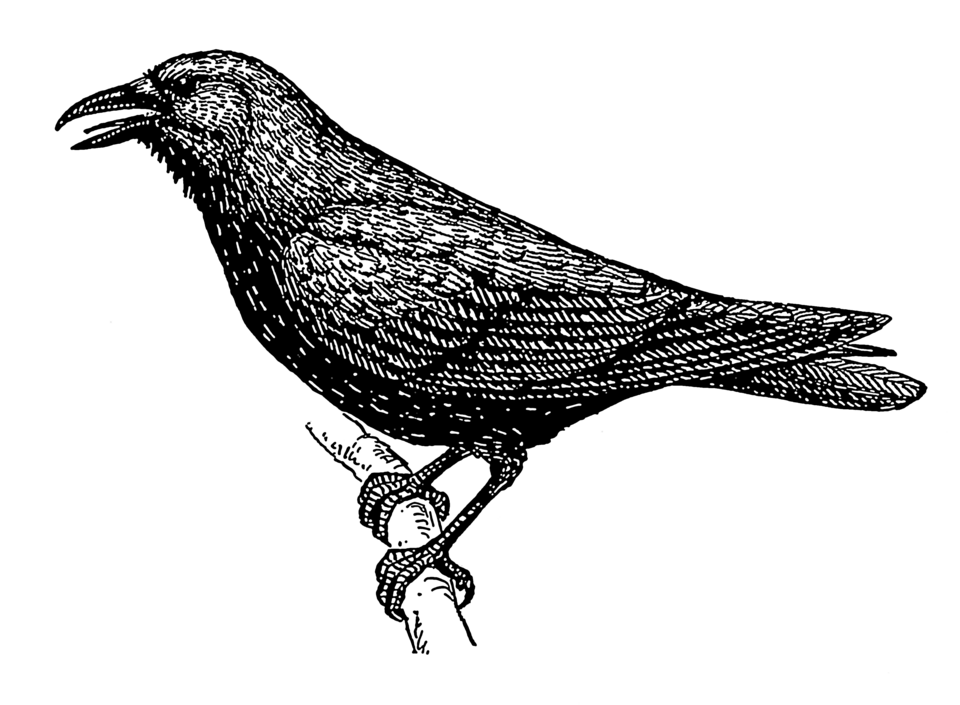
\includegraphics[width=12cm, height=4cm, keepaspectratio]{Billeder/Dyr/Fugle/Spurvefugle/spurvefugle.png}\\[1.2em]
    {\LARGE \textbf{Spurvefugle}}\\[0.6em]
    Artsbestemmelse \& vildtbiologi \\[0.9em]
    {\tiny\color{gray}
    CC BY 4.0 – kan frit anvendes, også kommercielt. Rettighederne må ikke skærpes.\\[0.05em]
    Udviklet af Aleksander Sønder, OSJAGTTEGN.DK}
  \end{center}
\end{frame}

\section{Spurvefugle/Kragefugle (vildtkending og biologi)}

% ========== SORTKRAGE ==========
\begin{frame}{%
  \begin{minipage}[c]{0.30\textwidth}
    Sortkrage (Krage)
  \end{minipage}%
  \hfill
  \begin{minipage}[c]{0.45\textwidth}
    \footnotesize
    \textbf{Jagttid:} 1.\ september -- 31.\ januar
  \end{minipage}%
  \hfill
  \begin{minipage}[c]{0.15\textwidth}
    \noindent\raggedleft
    
\includegraphics[width=0.5cm, height=0.5cm, keepaspectratio]{Billeder/Ikoner/star.png}%
    \hspace{0.2em}%
    
\includegraphics[width=0.5cm, height=0.5cm, keepaspectratio]{Billeder/Ikoner/star.png}%
    \hspace{0.2em}%
    
\includegraphics[width=0.5cm, height=0.5cm, keepaspectratio]{Billeder/Ikoner/star.png}
  \end{minipage}%
}
  \vspace{0.25em}
  \begin{columns}[T]
    \column{0.45\textwidth}
    \setlength{\parskip}{0.45em}
    \tiny
    \RaggedRight
    \textbf{\textit{Corvus corone}} – mellemstor kragefugl, nært beslægtet med gråkrage \par
    \textbf{Udseende:}\\
    \quad – Heltsort krop og hoved \\
    \quad – Sorte øjne \\
    \quad – Ligner ravn, men er mindre og har slankere næb \par
    \textbf{Levesteder:} Alle landskabstyper. \par
    \textbf{Føde:} Opportunist – spiser alt, inkl.\ yngel. \par
    \textbf{Udbredelse:} Især Vestjylland. Sjældnere i resten af landet. \par
    \textbf{Træk/standfugl:} Begge \par
    \textbf{Forplantning:}\\
    \quad – \textbf{Yngleforhold:} Yngler i høje træer. Parret forsvarer territoriet \\
    \quad – \textbf{Kønsmoden:} 2 år \\
    \quad – \textbf{Mono/polygam:} Monogam \\
    \quad – \textbf{Bestandsomsætning:} Langsom \\
    \quad – \textbf{Kuld:} 4--6 æg
    \column{0.52\textwidth}
    \centering
    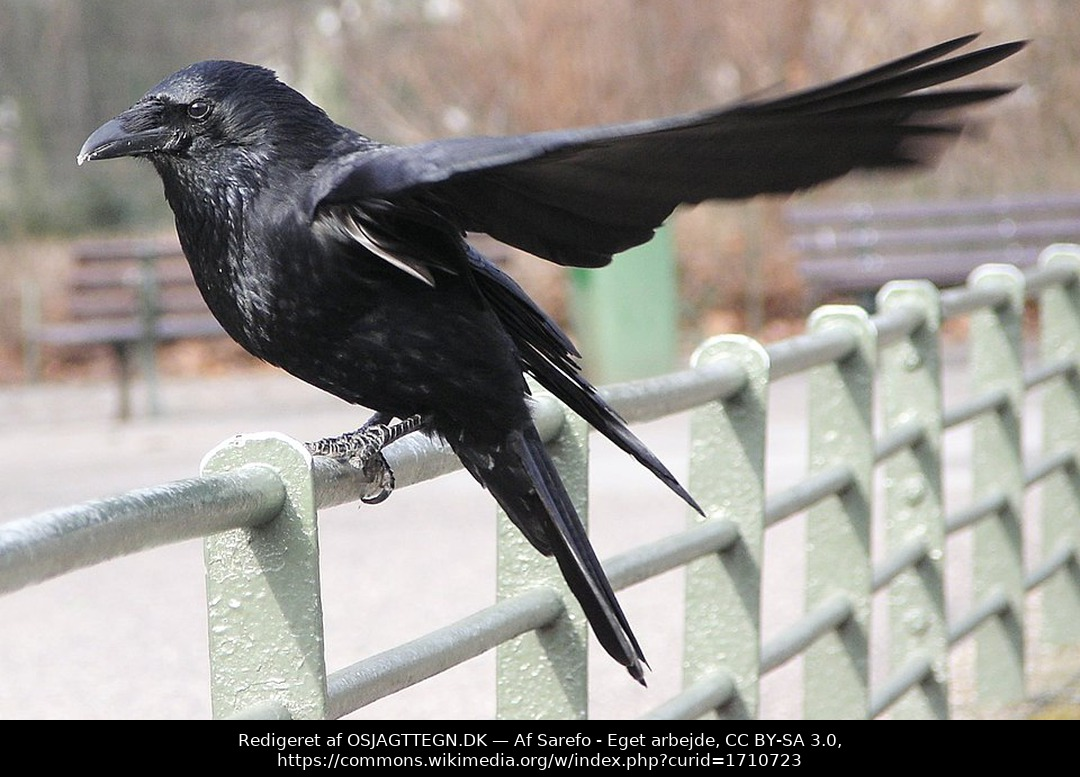
\includegraphics[width=\linewidth, height=7.2cm, keepaspectratio]{Billeder/Dyr/Fugle/Spurvefugle/sortkrage-01.jpg}
  \end{columns}
\end{frame}
% ========== GRÅKRAGE ==========
\begin{frame}{%
  \begin{minipage}[c]{0.30\textwidth}
    Gråkrage (Krage)
  \end{minipage}%
  \hfill
  \begin{minipage}[c]{0.45\textwidth}
    \footnotesize
    \textbf{Jagttid:} 1.\ september -- 31.\ januar
  \end{minipage}%
  \hfill
  \begin{minipage}[c]{0.15\textwidth}
    \noindent\raggedleft
    
\includegraphics[width=0.5cm, height=0.5cm, keepaspectratio]{Billeder/Ikoner/star.png}%
    \hspace{0.2em}%
    
\includegraphics[width=0.5cm, height=0.5cm, keepaspectratio]{Billeder/Ikoner/star.png}%
    \hspace{0.2em}%
    
\includegraphics[width=0.5cm, height=0.5cm, keepaspectratio]{Billeder/Ikoner/star.png}
  \end{minipage}%
}
  \vspace{0.25em}
  \begin{columns}[T]
    \column{0.45\textwidth}
    \setlength{\parskip}{0.45em}
    \tiny
    \RaggedRight
    \textbf{\textit{Corvus cornix}} – mellemstor kragefugl, den almindeligste krage i Danmark \par
    \textbf{Udseende:}\\
    \quad – Grå krop \\
    \quad – Sort hoved, bryst og vinger \\
    \quad – Sorte øjne \par
    \textbf{Levesteder:} Alle landskabstyper. \par
    \textbf{Føde:} Opportunist – spiser alt, inkl.\ yngel. \par
    \textbf{Udbredelse:} Hele Danmark. \par
    \textbf{Træk/standfugl:} Begge \par
    \textbf{Forplantning:}\\
    \quad – \textbf{Yngleforhold:} Yngler i høje træer. Parret forsvarer territoriet \\
    \quad – \textbf{Kønsmoden:} 2 år \\
    \quad – \textbf{Mono/polygam:} Monogam \\
    \quad – \textbf{Bestandsomsætning:} Langsom \\
    \quad – \textbf{Kuld:} 4--6 æg
    \column{0.52\textwidth}
    \centering
    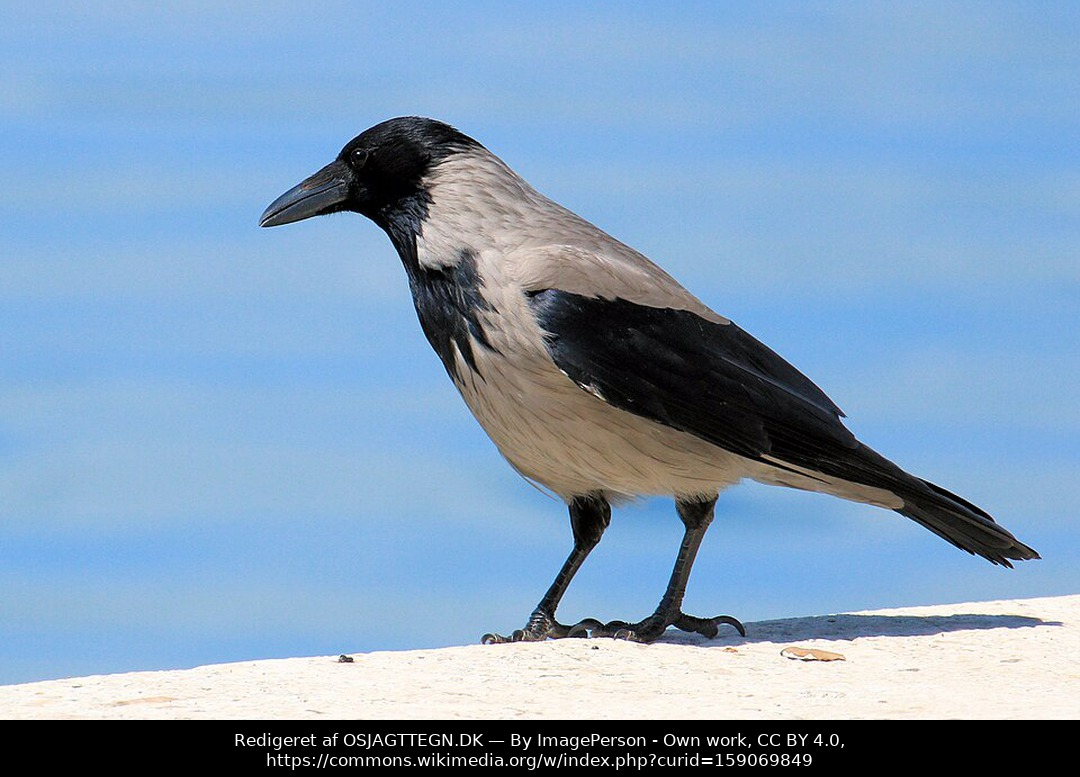
\includegraphics[width=\linewidth, height=7.2cm, keepaspectratio]{Billeder/Dyr/Fugle/Spurvefugle/graakrage-02.jpg}
  \end{columns}
\end{frame}

% ========== RAVN ==========
\begin{frame}{%
  \begin{minipage}[c]{0.30\textwidth}
    Ravn
  \end{minipage}%
  \hfill
  \begin{minipage}[c]{0.45\textwidth}
    \footnotesize
    \textbf{Jagttid:} Ingen jagttid
  \end{minipage}%
  \hfill
  \begin{minipage}[c]{0.15\textwidth}
    \noindent\raggedleft
    
\includegraphics[width=0.5cm, height=0.5cm, keepaspectratio]{Billeder/Ikoner/star.png}
  \end{minipage}%
}
  \vspace{0.25em}
  \begin{columns}[T]
    \column{0.45\textwidth}
    \setlength{\parskip}{0.5em}
    \tiny
    \RaggedRight
    \textbf{\textit{Corvus corax}} – stor, sort kragefugl med kraftigt næb \par
    \textbf{Udseende:}\\
    \quad – Heltsort fjerdragt \\
    \quad – Små fjer går ud på næbbet \\
    \quad – Kraftigere bygget end de øvrige kragefugle
    \column{0.52\textwidth}
    \centering
    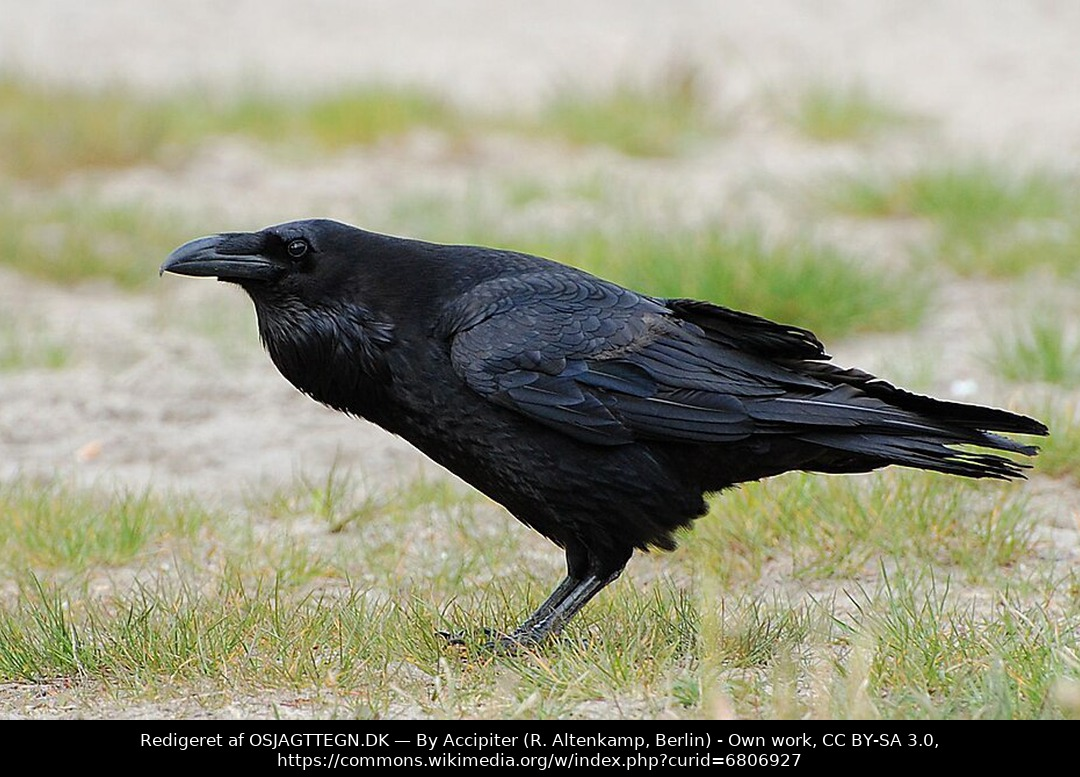
\includegraphics[width=\linewidth, height=7.2cm, keepaspectratio]{Billeder/Dyr/Fugle/Spurvefugle/ravn-01.jpg}
  \end{columns}
\end{frame}
% ========== RÅGE ==========
\begin{frame}{%
  \begin{minipage}[c]{0.30\textwidth}
    Råge
  \end{minipage}%
  \hfill
  \begin{minipage}[c]{0.45\textwidth}
    \footnotesize
    \textbf{Jagttid:} Ingen jagttid
  \end{minipage}%
  \hfill
  \begin{minipage}[c]{0.15\textwidth}
    \noindent\raggedleft
    
\includegraphics[width=0.5cm, height=0.5cm, keepaspectratio]{Billeder/Ikoner/star.png}%
    \hspace{0.2em}%
    
\includegraphics[width=0.5cm, height=0.5cm, keepaspectratio]{Billeder/Ikoner/star.png}
  \end{minipage}%
}
  \vspace{0.25em}
  \begin{columns}[T]
    \column{0.45\textwidth}
    \setlength{\parskip}{0.5em}
    \tiny
    \RaggedRight
    \textbf{\textit{Corvus frugilegus}} – kolonirugende kragefugl med fjerløs næbrod \par
    \textbf{Udseende:}\\
    \quad – Sort med metallisk skær \\
    \quad – Bart, gult eller gråligt parti ved næbbets rod \par
    \textbf{Levesteder:} Alle landskabstyper, men hyppigere ved byer. \par
    \textbf{Føde:} Plantemateriale suppleret med insekter og lignende. \par
    \textbf{Udbredelse:} Hele Danmark. \par
    \textbf{Træk/standfugl:} Standfugl
    \column{0.52\textwidth}
    \centering
    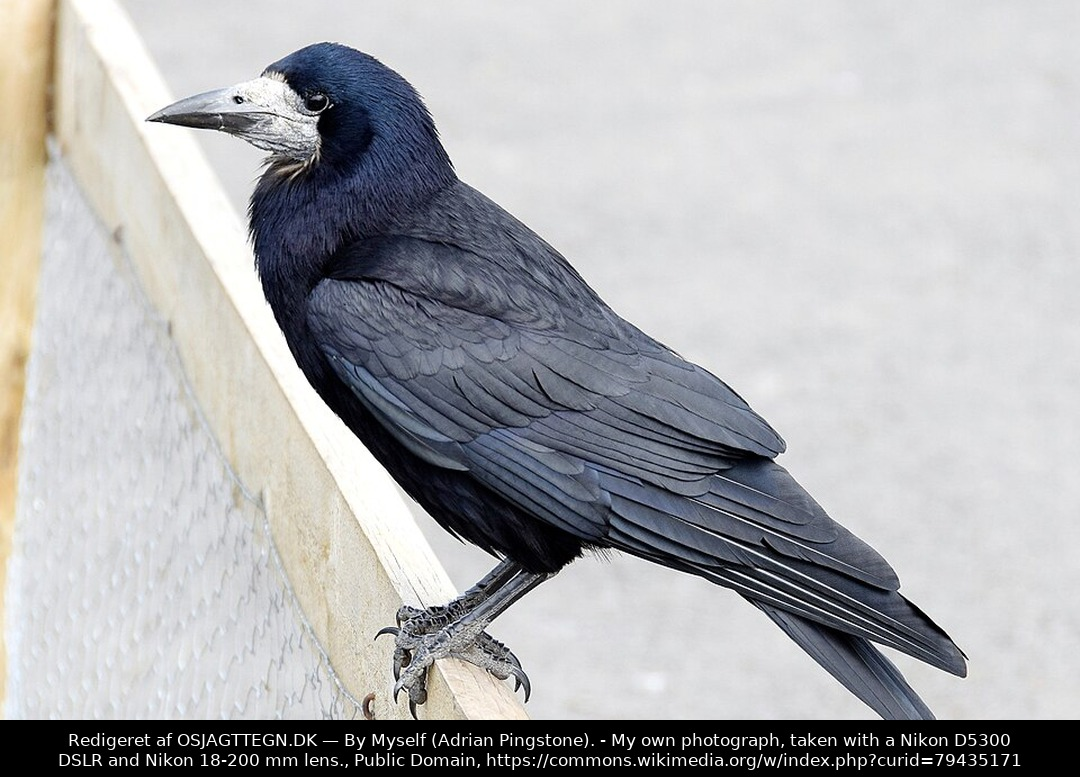
\includegraphics[width=\linewidth, height=7.2cm, keepaspectratio]{Billeder/Dyr/Fugle/Spurvefugle/raage-01.jpg}
  \end{columns}
\end{frame}
% ========== ALLIKE ==========
\begin{frame}{%
  \begin{minipage}[c]{0.30\textwidth}
    Allike
  \end{minipage}%
  \hfill
  \begin{minipage}[c]{0.45\textwidth}
    \footnotesize
    \textbf{Jagttid:} Ingen jagttid
  \end{minipage}%
  \hfill
  \begin{minipage}[c]{0.15\textwidth}
    \noindent\raggedleft
    
\includegraphics[width=0.5cm, height=0.5cm, keepaspectratio]{Billeder/Ikoner/star.png}
  \end{minipage}%
}
  \vspace{0.25em}
  \begin{columns}[T]
    \column{0.45\textwidth}
    \setlength{\parskip}{0.5em}
    \tiny
    \RaggedRight
    \textbf{\textit{Coloeus monedula}} – mindste kragefugl i Danmark med hvidgule øjne \par
    \textbf{Udseende:}\\
    \quad – Mindre end de andre kragefugle \\
    \quad – Grå nakke og hals \\
    \quad – Kendes især på det hvidgule øje
    \column{0.52\textwidth}
    \centering
    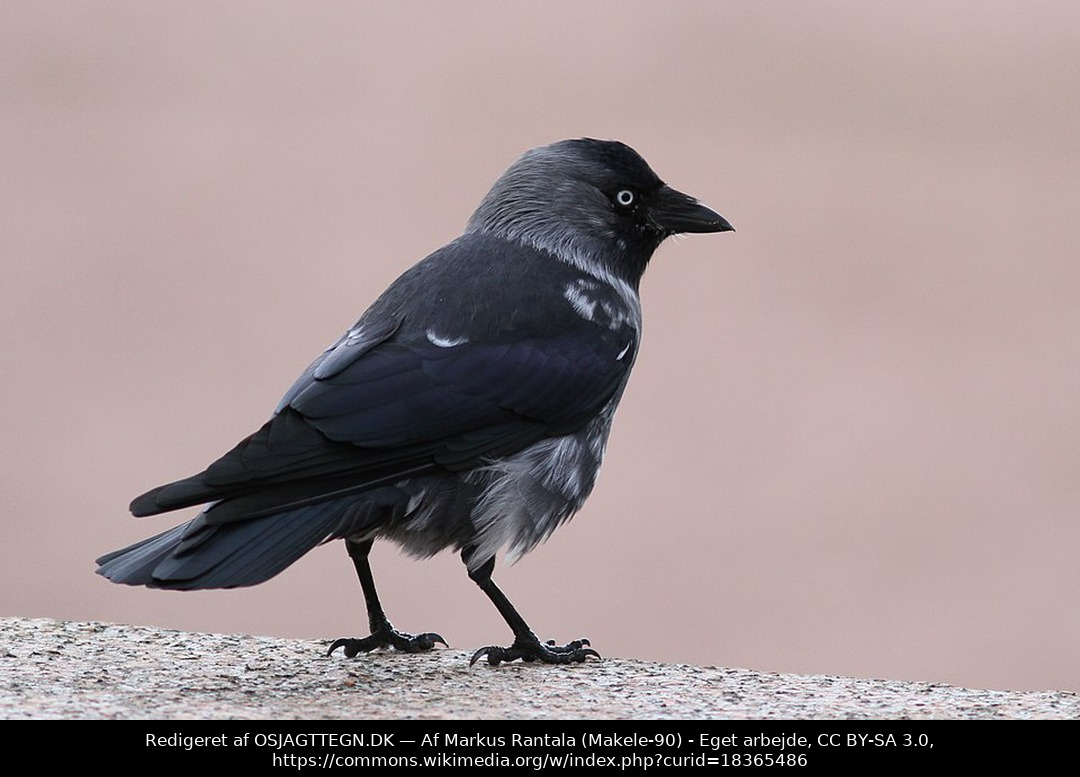
\includegraphics[width=\linewidth, height=7.2cm, keepaspectratio]{Billeder/Dyr/Fugle/Spurvefugle/allike-01.jpg}
  \end{columns}
\end{frame}
% ========== HUSSKADE ==========
\begin{frame}{%
  \begin{minipage}[c]{0.30\textwidth}
    Husskade
  \end{minipage}%
  \hfill
  \begin{minipage}[c]{0.45\textwidth}
    \footnotesize
    \textbf{Jagttid:} 1.\ september -- 31.\ januar
  \end{minipage}%
  \hfill
  \begin{minipage}[c]{0.15\textwidth}
    \noindent\raggedleft
    
\includegraphics[width=0.5cm, height=0.5cm, keepaspectratio]{Billeder/Ikoner/star.png}%
    \hspace{0.2em}%
    
\includegraphics[width=0.5cm, height=0.5cm, keepaspectratio]{Billeder/Ikoner/star.png}
  \end{minipage}%
}
  \vspace{0.25em}
  \begin{columns}[T]
    \column{0.45\textwidth}
    \setlength{\parskip}{0.5em}
    \tiny
    \RaggedRight
    \textbf{\textit{Pica pica}} – kendes på den lange hale og den sort-hvide fjerdragt \par
    \textbf{Udseende:}\\
    \quad – Sort og hvid med blågrønne metalskær \\
    \quad – Hoved og ryg sorte \\
    \quad – Bug og dele af vingerne hvide \par
    \textbf{Levesteder:} Alle landskabstyper, oftest i bynære zoner. \par
    \textbf{Føde:} Altædende. \par
    \textbf{Udbredelse:} Hele Danmark. \par
    \textbf{Træk/standfugl:} Standfugl
    \column{0.52\textwidth}
    \centering
    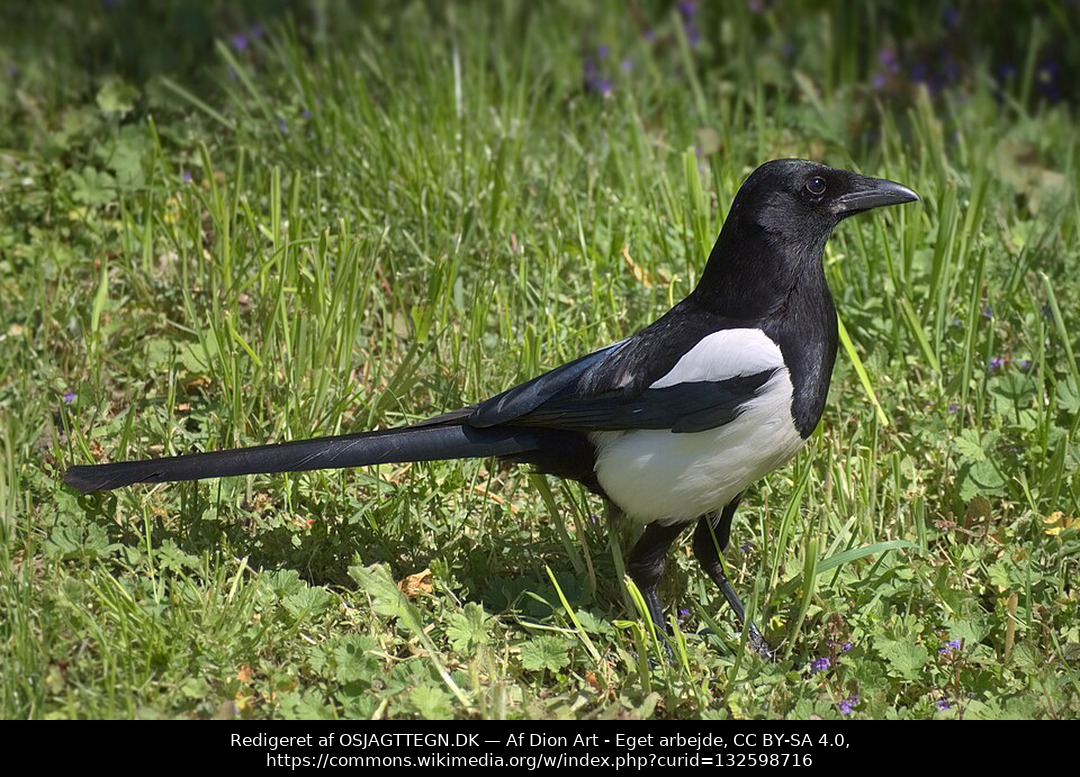
\includegraphics[width=\linewidth, height=7.2cm, keepaspectratio]{Billeder/Dyr/Fugle/Spurvefugle/husskade-01.jpg}
  \end{columns}
\end{frame}
% ========== SKOVSKADE ==========
\begin{frame}{%
  \begin{minipage}[c]{0.30\textwidth}
    Skovskade
  \end{minipage}%
  \hfill
  \begin{minipage}[c]{0.45\textwidth}
    \footnotesize
    \textbf{Jagttid:} Ingen jagttid
  \end{minipage}%
  \hfill
  \begin{minipage}[c]{0.15\textwidth}
    \noindent\raggedleft
    
\includegraphics[width=0.5cm, height=0.5cm, keepaspectratio]{Billeder/Ikoner/star.png}
  \end{minipage}%
}
  \vspace{0.25em}
  \begin{columns}[T]
    \column{0.45\textwidth}
    \setlength{\parskip}{0.5em}
    \tiny
    \RaggedRight
    \textbf{\textit{Garrulus glandarius}} – kendes på den rødbrune fjerdragt og det lyseblå felt på vingen \par
    \textbf{Udseende:}\\
    \quad – Rødbrun med hvid strube \\
    \quad – Sort hale \\
    \quad – Lyseblåt felt med sorte striber på vingen
    \column{0.52\textwidth}
    \centering
    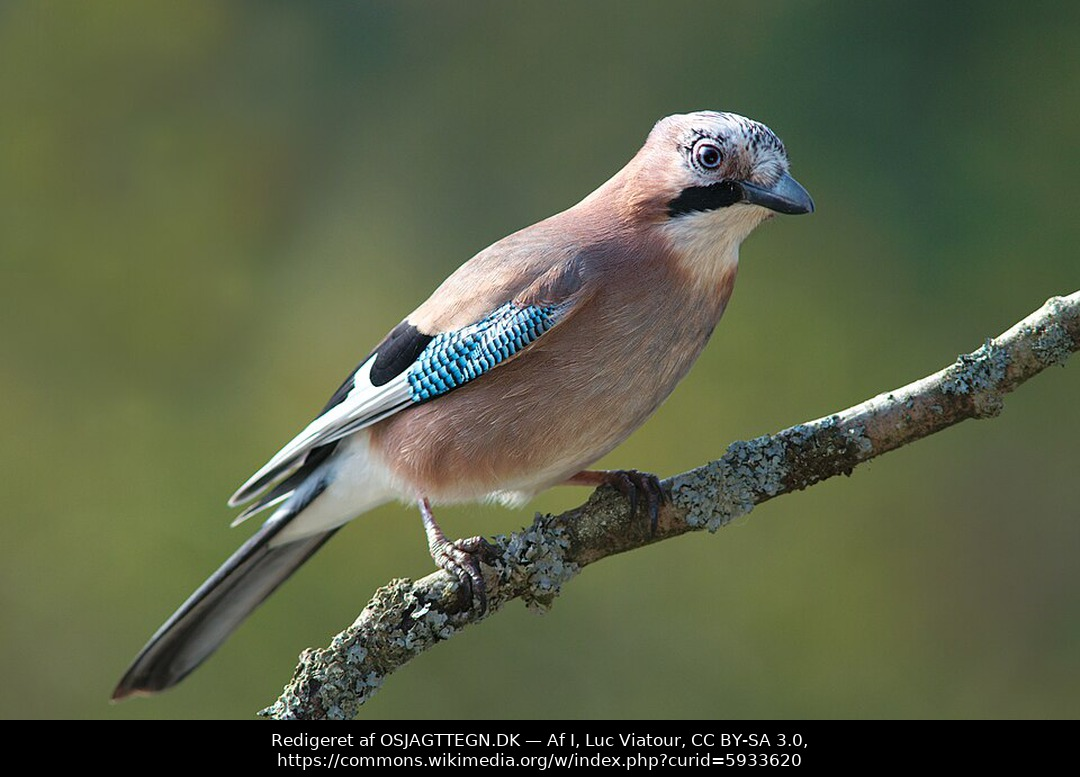
\includegraphics[width=\linewidth, height=7.2cm, keepaspectratio]{Billeder/Dyr/Fugle/Spurvefugle/skovskade-01.jpg}
  \end{columns}
\end{frame}

\begin{frame}
  \vspace{1.8em}
  \begin{center}
    \begin{minipage}{0.22\textwidth}
      \centering
      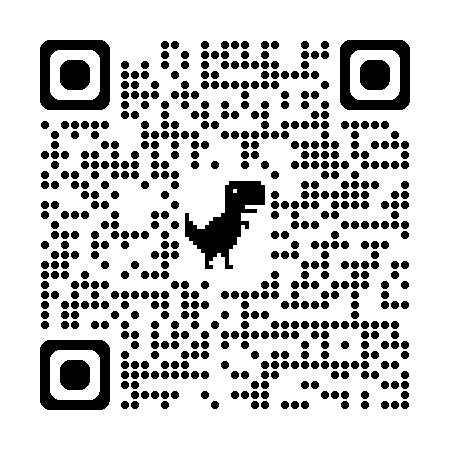
\includegraphics[width=\linewidth]{Billeder/Dyr/Fugle/Spurvefugle/qr/spurvefugle_qr.png}
    \end{minipage}%
    \hspace{0.8em}%
    \begin{minipage}{0.62\textwidth}
      \raggedright
      \Large
      \textbf{Træning i artsbestemmelse af spurvefugle}\\[0.35em]
      {\large https://osjagttegn.dk/spurvefugle}
    \end{minipage}
  \end{center}
\end{frame}